% Created 2026-04-23 Thu 12:08
% Intended LaTeX compiler: lualatex
\DocumentMetadata{lang = en-US,pdfversion = 2.0,pdfstandard = ua-2,tagging = on,tagging-setup = {math/setup=mathml-SE},}
\documentclass[11pt]{article}
\usepackage{amsmath}
\usepackage{fontspec}
\usepackage{graphicx}
\usepackage{longtable}
\usepackage{wrapfig}
\usepackage{rotating}
\usepackage[normalem]{ulem}
\usepackage{capt-of}
\usepackage{hyperref}
\usepackage[margin=1in]{geometry}
\usepackage{fontspec}
\usepackage{verbatim, multicol, tabularx,}
\usepackage{amsmath, amsthm, amssymb, stmaryrd, latexsym, bm, listings, qtree}
\usepackage{framed}
\usepackage{xcolor,colortbl}
\usepackage{media9}
\usepackage[export]{adjustbox}
\usepackage{algorithm}
\usepackage[noend]{algpseudocode}
\usepackage{tikz,pgfplots}
\usetikzlibrary{shapes.geometric}
\let\oldquote=\quote
\let\endoldquote=\endquote
\colorlet{shadecolor}{cyan!15}
\renewenvironment{quote}{\begin{shaded*}\begin{oldquote}}{\end{oldquote}\end{shaded*}}
% From https://tex.stackexchange.com/questions/7032/good-way-to-make-textcircled-numbers
\newcommand*\circled[1]{\tikz[baseline=(char.base)]{\node[shape=circle,draw,inner sep=2pt] (char) {#1};}}
\DeclareMathOperator*{\argmin}{arg\!min}
\DeclareMathOperator*{\argmax}{arg\!max}
\lstset{frame=tb, aboveskip=1mm, belowskip=0mm, showstringspaces=false, columns=flexible, basicstyle={\scriptsize\ttfamily}, numbers=left, frame=single, breaklines=true, breakatwhitespace=true}
\hypersetup{colorlinks=true,urlcolor=blue}
\usepackage{tagpdf}
\tagpdfsetup{activate-all}
\tagpdfsetup{math/alt/use}
\usepackage{polyglossia}
\setdefaultlanguage[variant=en-US]{english}
\author{Artificial Intelligence}
\date{Christopher Simpkins}
\title{Intelligent Agents\\\medskip
\large Artificial Intelligence}
\hypersetup{
 pdfauthor={Artificial Intelligence},
 pdftitle={Intelligent Agents},
 pdfkeywords={},
 pdfsubject={Intelligent Agents Artificial Intelligence},
 pdfcreator={Emacs 30.2 (Org mode 9.7.11)}, 
 pdflang={English}}
\begin{document}

\maketitle
\section{What is an agent?}
\label{sec:orga405457}



\includegraphics[alt={agent smith subway fight},height=3.2in]{agent-smith-subway-fight.jpg}



\href{https://x.com/aist\_digital/status/1954905895025942918}{https://x.com/aist\textsubscript{digital}/status/1954905895025942918}
\section{Agents}
\label{sec:org10fc745}


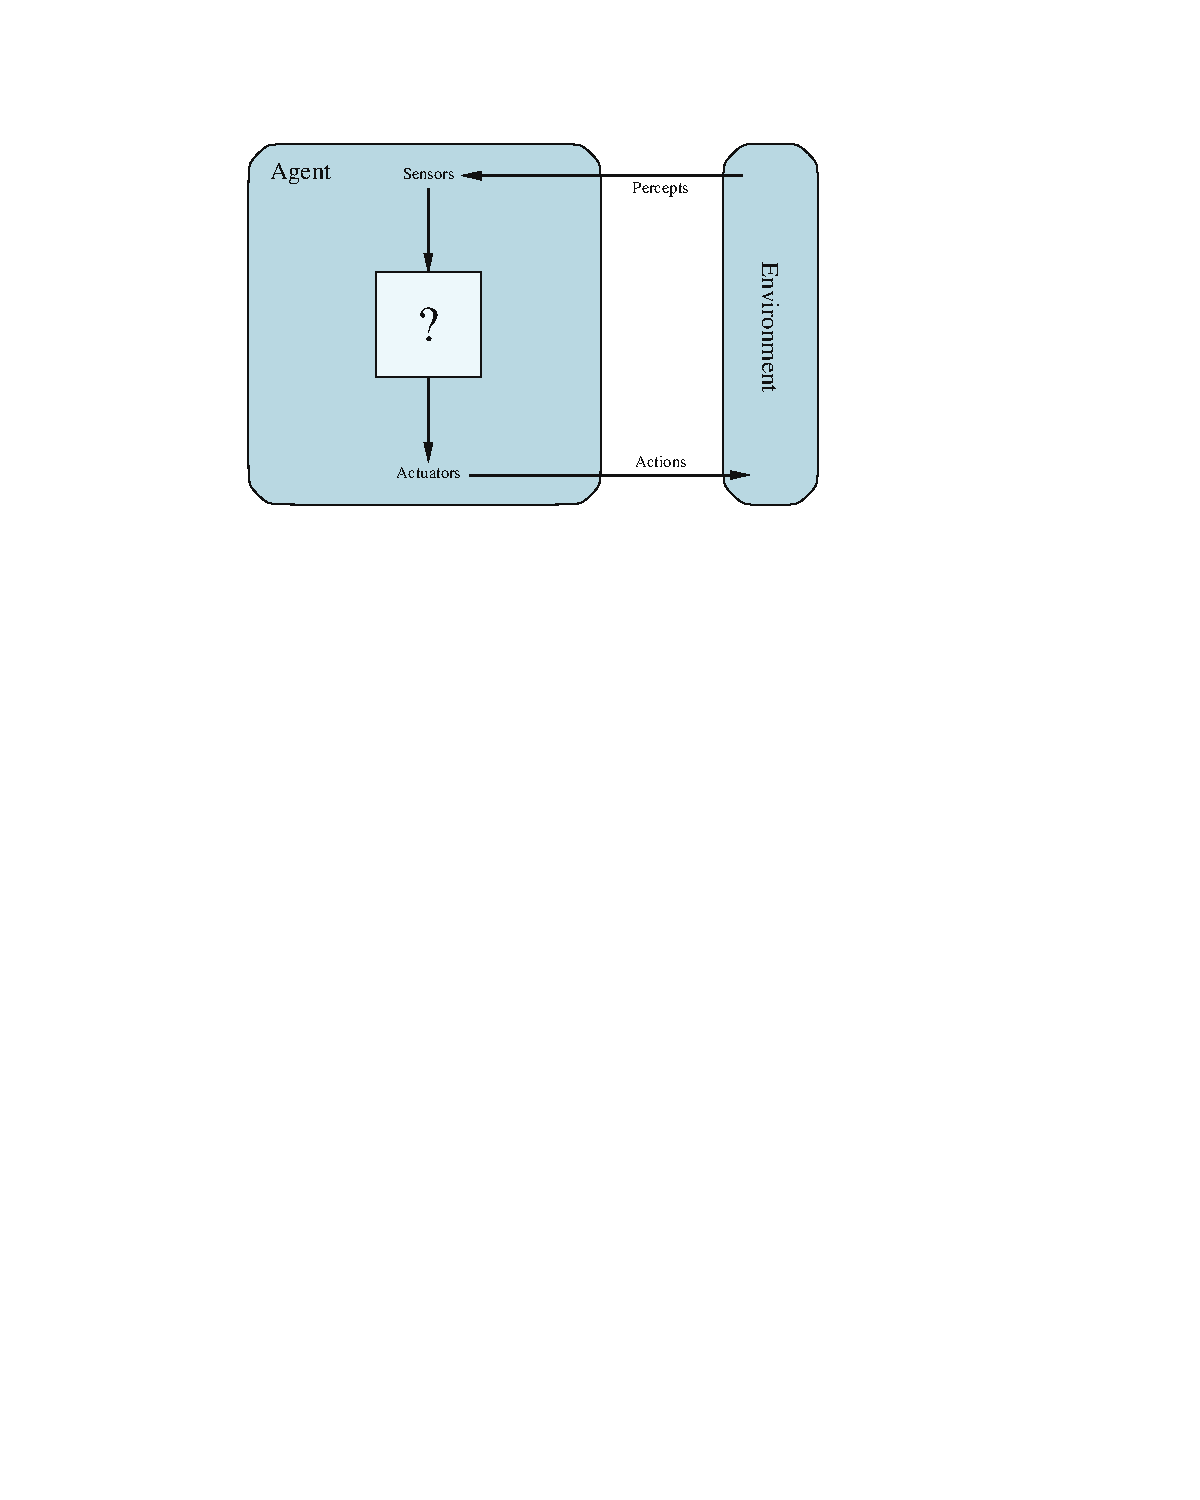
\includegraphics[alt={aima fig 02_01 agent environment},width=0.75\linewidth]{aima-fig-02_01-agent-environment.pdf}
\section{Agent Functions}
\label{sec:orgccb3bd0}

An \textbf{agent function} is an external tabulation of the agent's behavior.


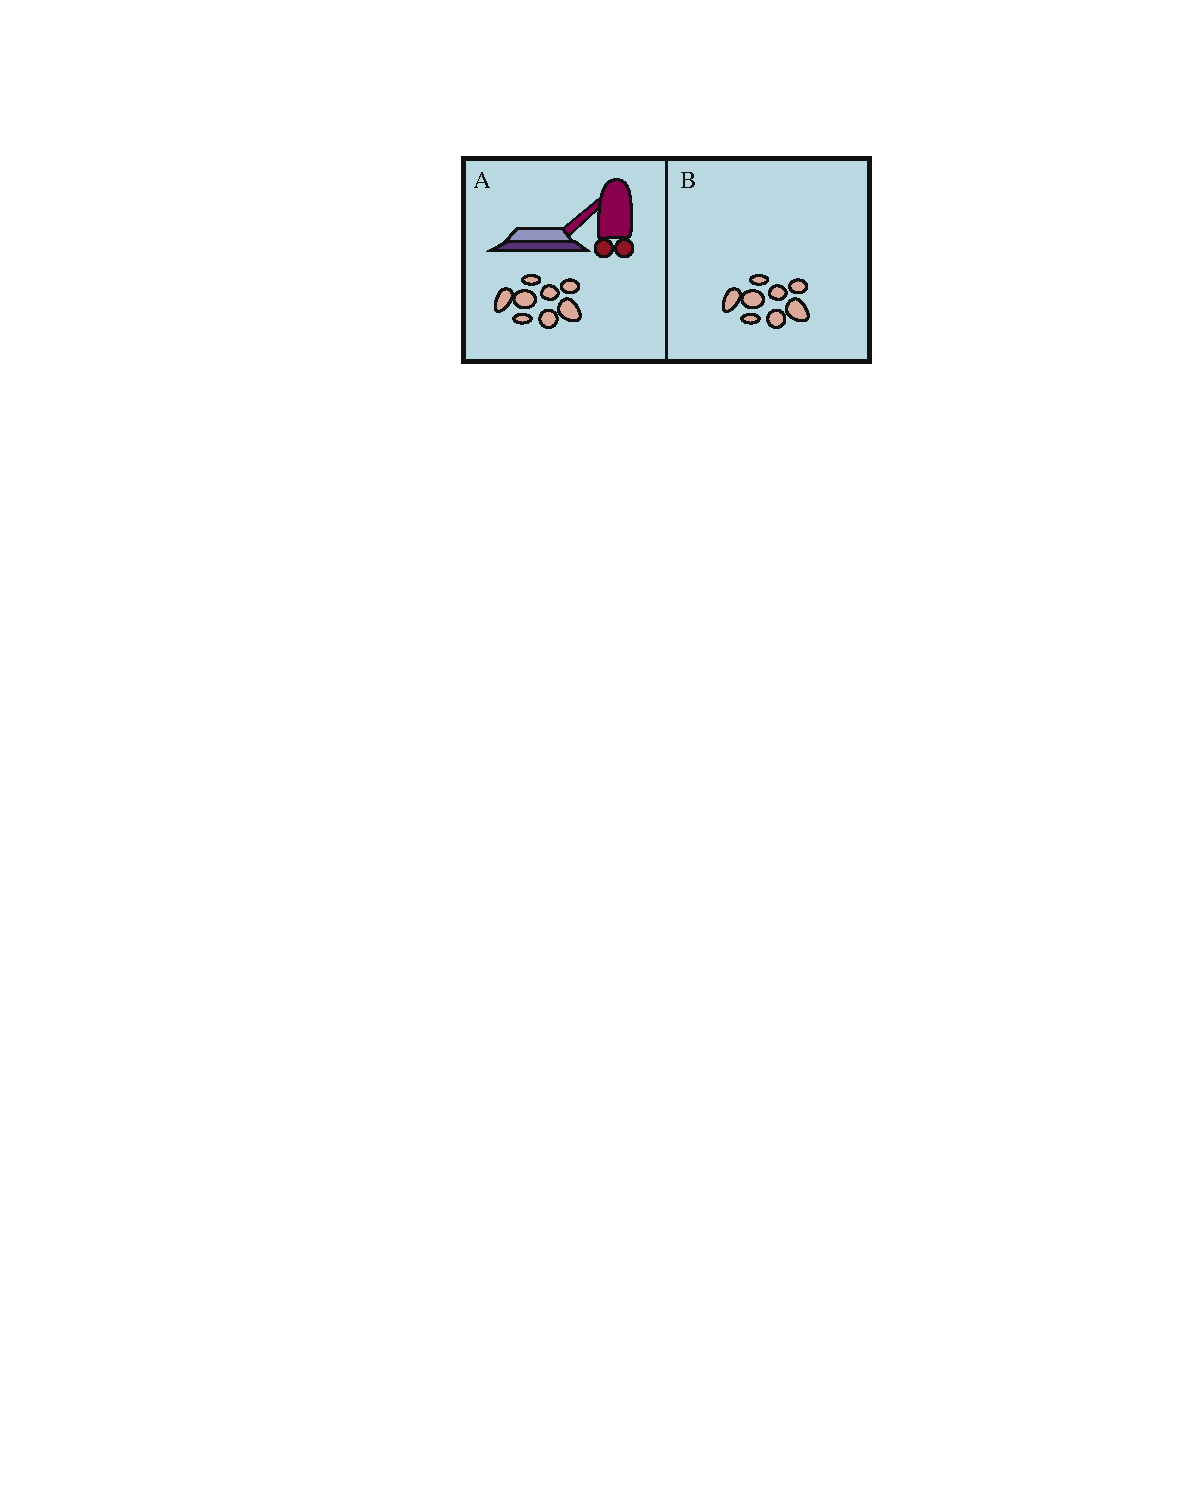
\includegraphics[alt={aima fig 02_02 vacuum world},height=0.6in]{aima-fig-02_02-vacuum-world.pdf}
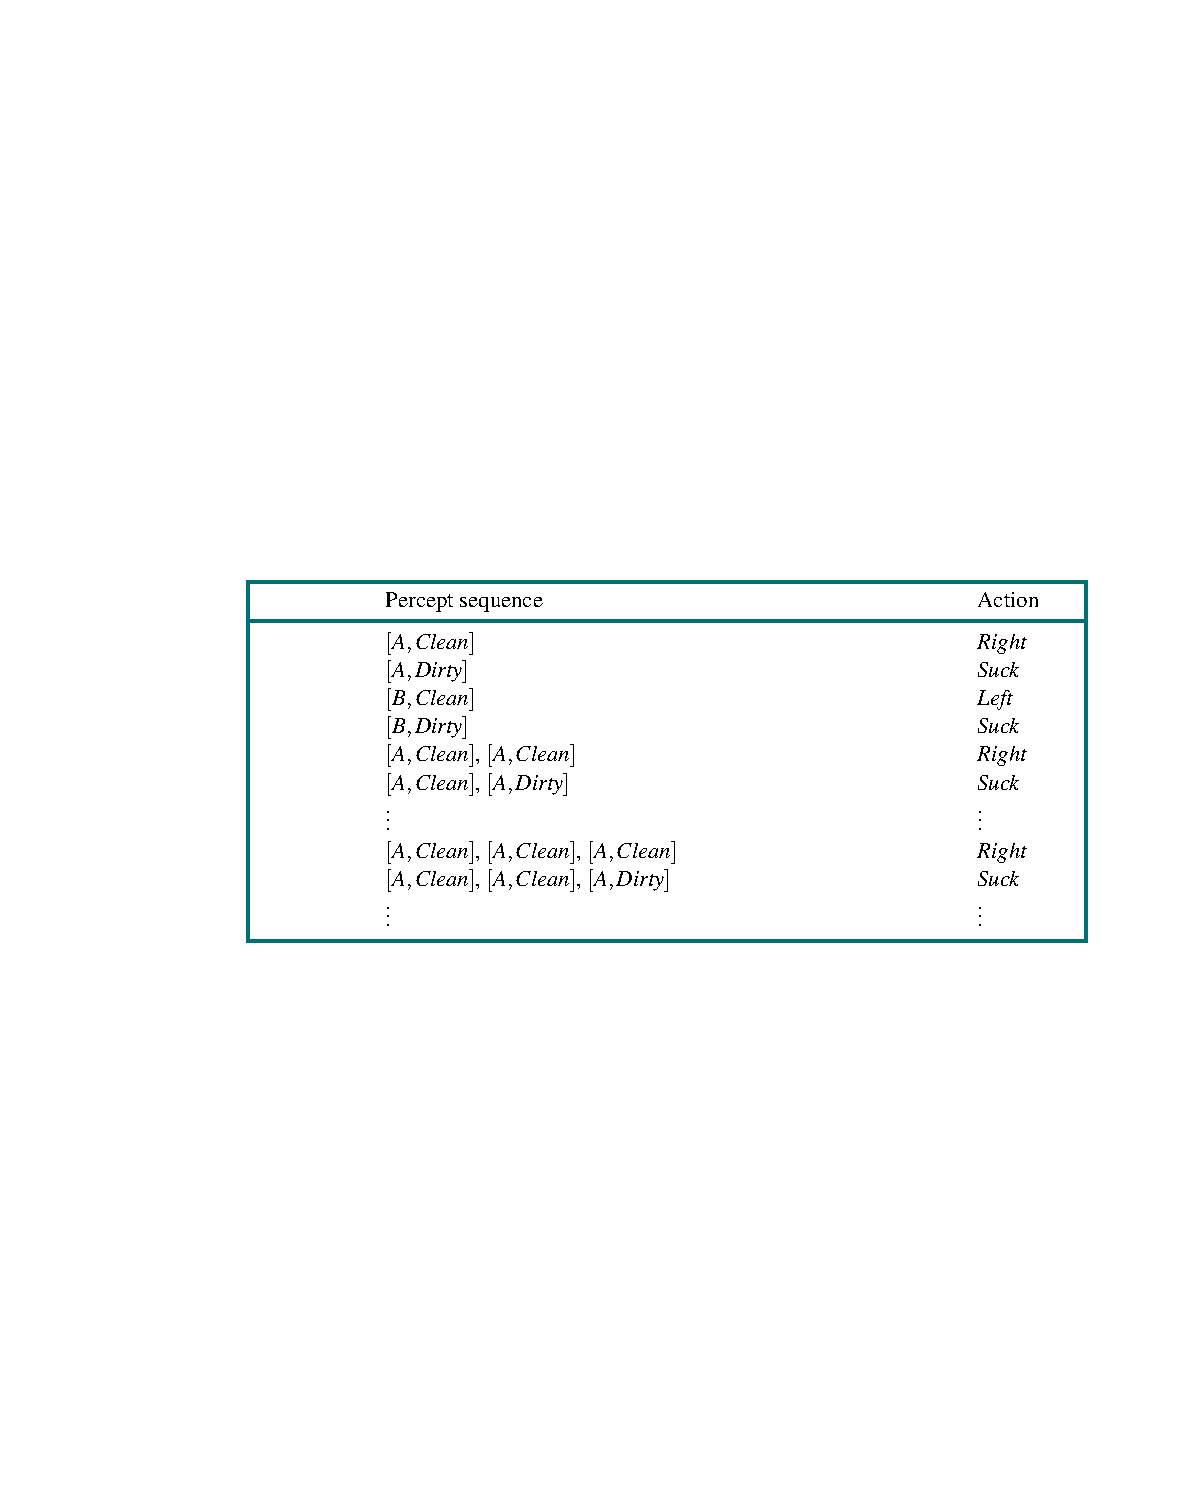
\includegraphics[alt={aima fig 02_03 vacuum function},height=3.0in]{aima-fig-02_03-vacuum-function.pdf}


An \textbf{agent program} is an implementation of an agent function inside the agent.
\section{Intelligent Agents}
\label{sec:orgac135ef}

An intelligent agent is \textbf{rational}.  Rationality \ldots{}

\begin{itemize}
\item is consequentialist.

\begin{itemize}
\item We judge behavior as rational if it leads to desirable consequences.
\end{itemize}

\item needs an external \textbf{performance measure} to make this judgment.
\end{itemize}

Beware of the Genie effect.

\begin{itemize}
\item Example: what if our performance measure is "amount of dirt sucked up?"
\end{itemize}

\begin{quote}
Performance measures should specify desired states of the environment, not preconceived notions of what the agent's behavior should be.
\end{quote}
\section{Rationality}
\label{sec:org157e8aa}

Judgment of rationality depends on:

\begin{itemize}
\item The performance measure that defines the criterion of success.
\item The agent’s prior knowledge of the environment.
\item The actions that the agent can perform.
\item The agent’s percept sequence to date.
\end{itemize}

Now we can define \textbf{rational agent}:

\begin{quote}
For each possible percept sequence, a rational agent should select an action that is expected to maximize its performance measure, given the evidence provided by the percept sequence and whatever built-in knowledge the agent has.
\end{quote}

Note that the performance measure is external to the agent, representing a general notion of "success" within an environment that applies to any agent in the environment.
\section{Omniscience, Rationality, Learning and Autonomy}
\label{sec:org60cea52}

Omniscience: for a given state and action, agent knows the result state exactly.

\begin{itemize}
\item Omniscience is impossible in practice
\item Rationality means choosing the best action given what you know, i.e., the percept sequence to date.
\end{itemize}

Key idea: how to maximize the usefulness of the agent's percept sequence.

\begin{itemize}
\item Information gathering, exploration.
\item Learning makes use of exploration.
\item Prior knowledge.
\end{itemize}

The more an agent is able to learn, the more autonomy it has.
\section{Task Environments}
\label{sec:org47e60c0}

The concept of an environment is both general and limited.  In AI we are usually interested in a particular task within an environment.  We call these \textbf{task environments} and they represent the "problems" that an intelligent agent "solves."

Task environment specification: PEAS

\begin{itemize}
\item *P*erformance measure
\item *E*nvironment dynamics -- what is the result of applying an action
\item *A*ctuators to modify the environment
\item *S*ensors to perceive the environment
\end{itemize}

Notice that there is a blurring of the line between what we intuitively consider an \textbf{agent} versus the \textbf{environment} in which it acts.
\section{Taxi Task Environment}
\label{sec:orgc91f0e3}


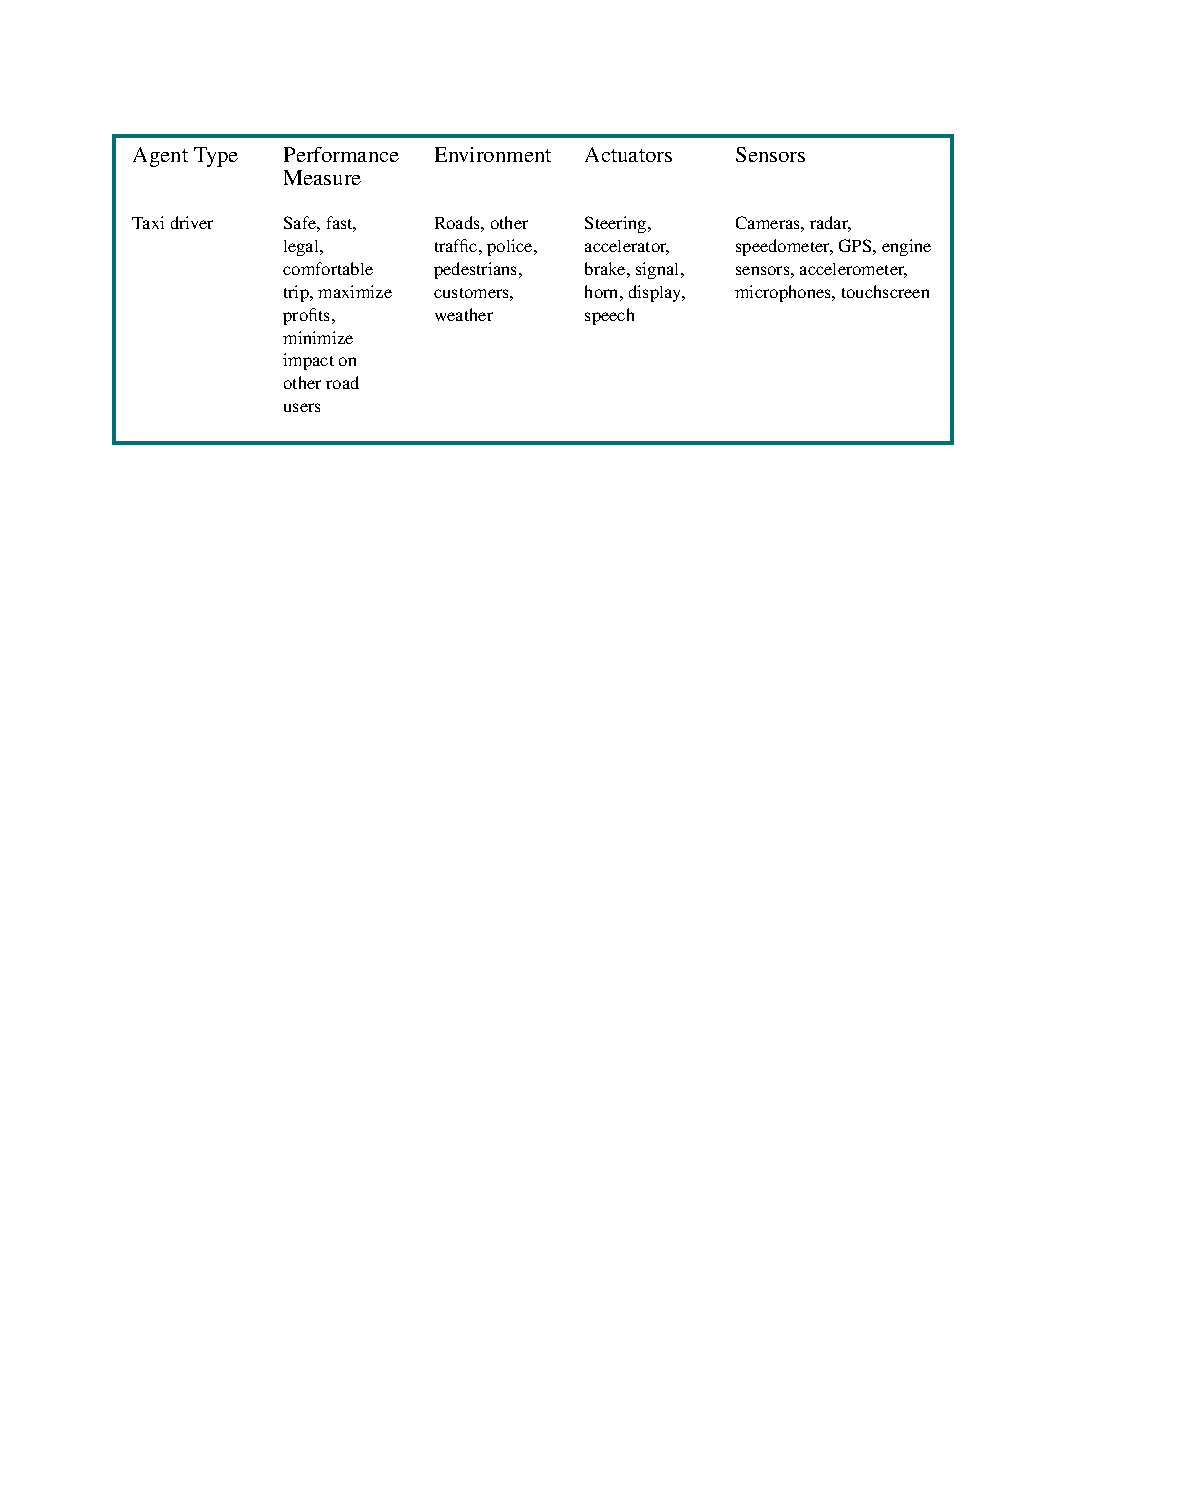
\includegraphics[alt={aima fig 02_04 taxi task environment},width=0.75\linewidth]{aima-fig-02_04-taxi-task-environment.pdf}
\section{Example Agent Types and Their PEAS Descriptions}
\label{sec:orgfdae0e5}


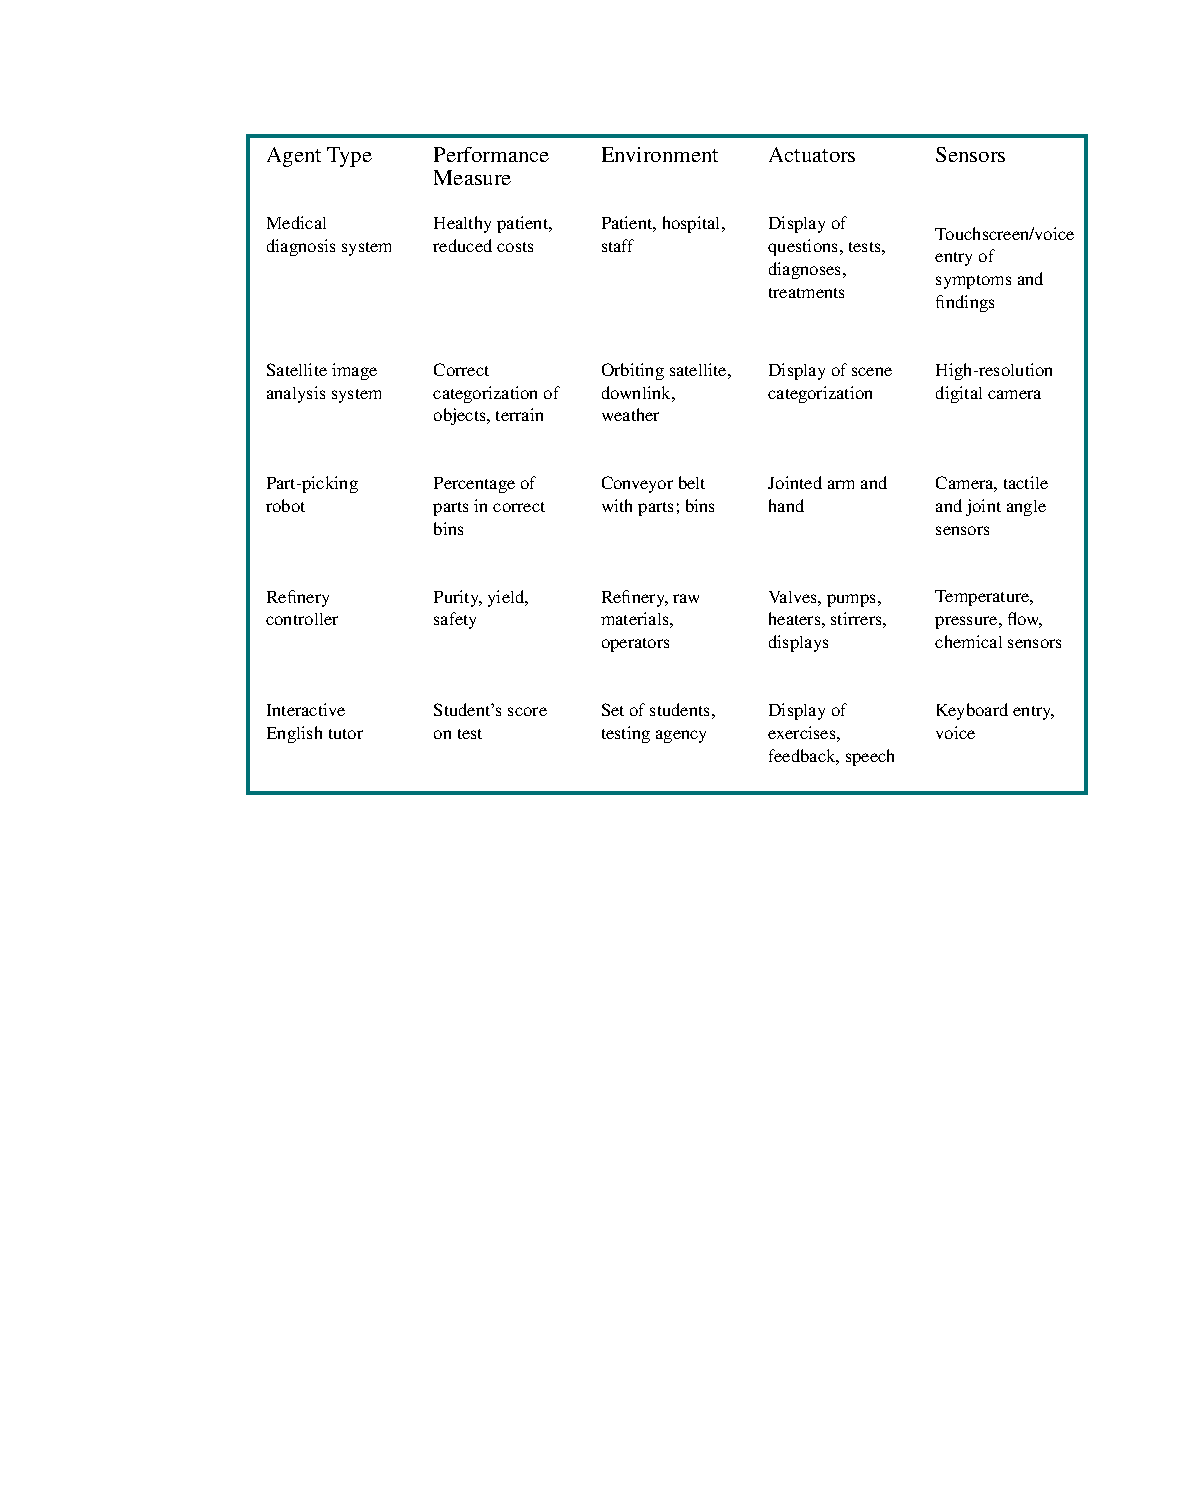
\includegraphics[alt={aima fig 02_05 agent types},height=3.6in]{aima-fig-02_05-agent-types.pdf}
\section{Task Environment Design Space}
\label{sec:orgdd049b2}

\begin{itemize}
\item Fully vs. partially observable
\item Single agent vs. multi-agent
\begin{itemize}
\item Competitive vs. cooperative
\end{itemize}
\item Deterministic vs. nondeterministic
\begin{itemize}
\item Stochastic is a specific kind of nondeterminism in which we assign probabilities to outcomes
\end{itemize}
\item Episodic vs. sequential
\begin{itemize}
\item Episodic: current action independent of previous decisions and future decisions
\item Sequential: current action may affect all future actions
\end{itemize}
\item Static vs. dynamic
Can the environment change while agent is deliberating?
\item Discrete vs. continuous
\item Known vs. unknown
\begin{itemize}
\item Does the agent know the "physics" of the environment?
\end{itemize}
\end{itemize}
\section{Task Environment Examples}
\label{sec:orgcfab617}


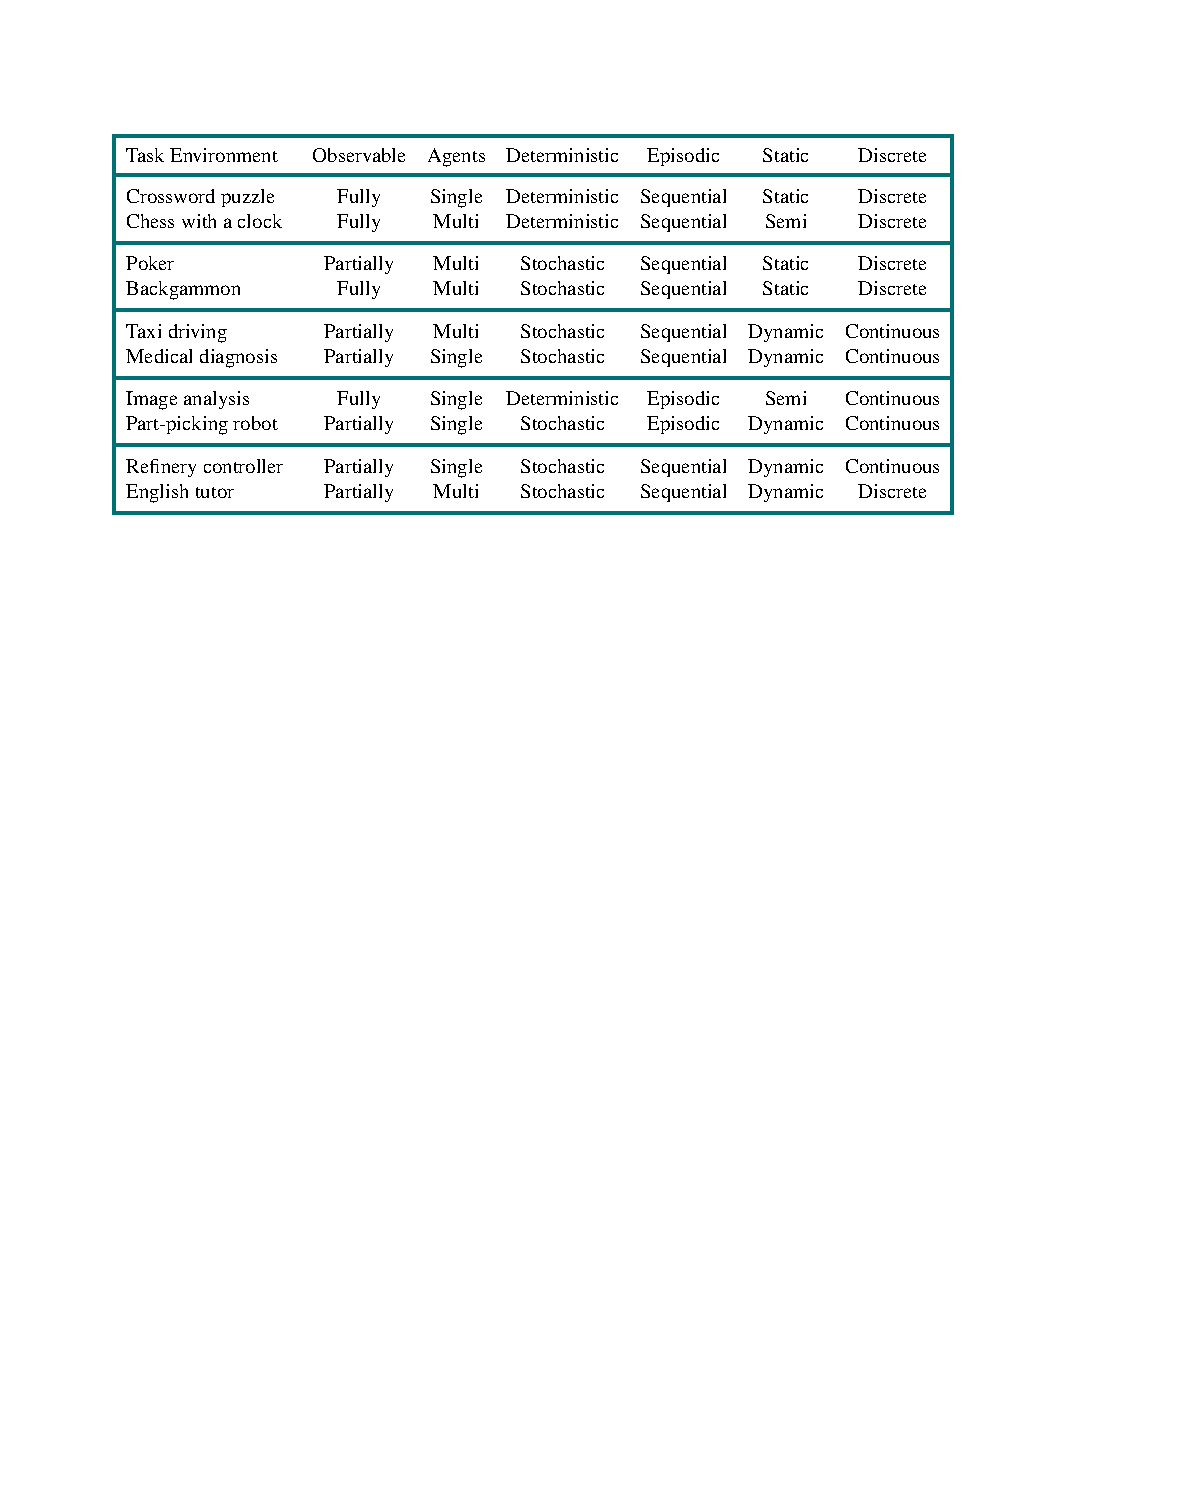
\includegraphics[alt={aima fig 02_06 example tasks},height=3.6in]{aima-fig-02_06-example-tasks.pdf}
\section{The Structure of Agents}
\label{sec:org6da5c59}

\begin{itemize}
\item An \textbf{agent program} is an implementation of an agent function inside the agent.
\item An \textbf{agent architecture} is the computing device on which the agent runs, including sensors and actuators (which may be virtual).
\begin{itemize}
\item When we put an agent program inside a physical platform, like a robot, we call it \textbf{embodied intelligence}.
\end{itemize}
\end{itemize}

\begin{equation*}
agent = architecture + program
\end{equation*}

This entire course, indeed all of AI, is about designing intelligent agents.
\section{Table-driven Agent}
\label{sec:orgf825f97}

A table-driven agent program implements the agent function directly.



\includegraphics[alt={aima fig 02_07 table driven agent program},width=0.75\linewidth]{aima-fig-02_07-table-driven-agent-program.pdf}


If \(\mathcal{P}\) is the set of possible percepts and \(T\) is the lifetime of the agent, then the size of the agent table is impossibly large in practice:

\vspace{-.2in}
$$
\sum_{t=1}^T |\mathcal{P}|^t
$$

\begin{quote}
Key idea: a full representation of the ideal agent program is usually impossible in practice.  Our job as AI agent developers is to design a compact representation of the ideal agent program.
\end{quote}
\section{Reflex Vacuum Agent}
\label{sec:org7fa1f6e}


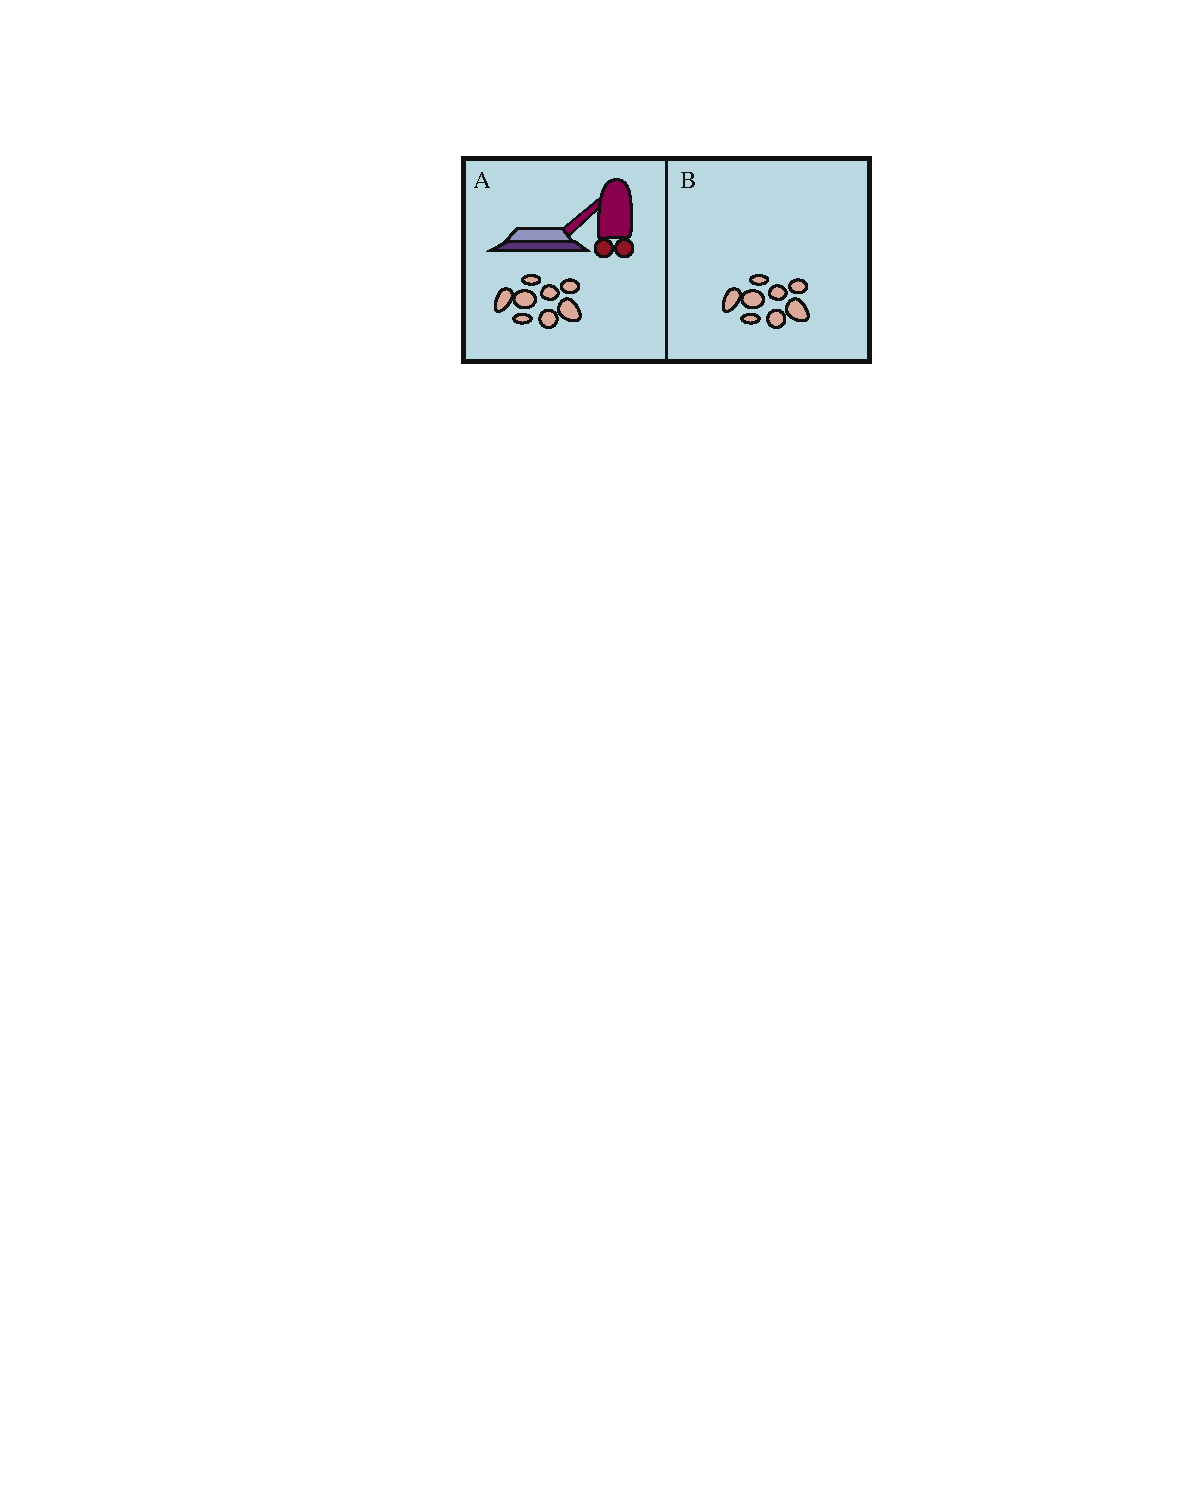
\includegraphics[alt={aima fig 02_02 vacuum world},width=0.75\linewidth]{aima-fig-02_02-vacuum-world.pdf}


\includegraphics[alt={aima fig 02_08 reflex vacuum agent program},width=0.75\linewidth]{aima-fig-02_08-reflex-vacuum-agent-program.pdf}
\section{General Reflex Agents}
\label{sec:org07f18e7}

\begin{flushleft}
#+latex: 
\includegraphics[alt={aima fig 02_10 reflex agent program},width=0.75\linewidth]{aima-fig-02_10-reflex-agent-program.pdf}
\end{flushleft}

\vspace{-.2in}
\begin{flushright}
#+latex: 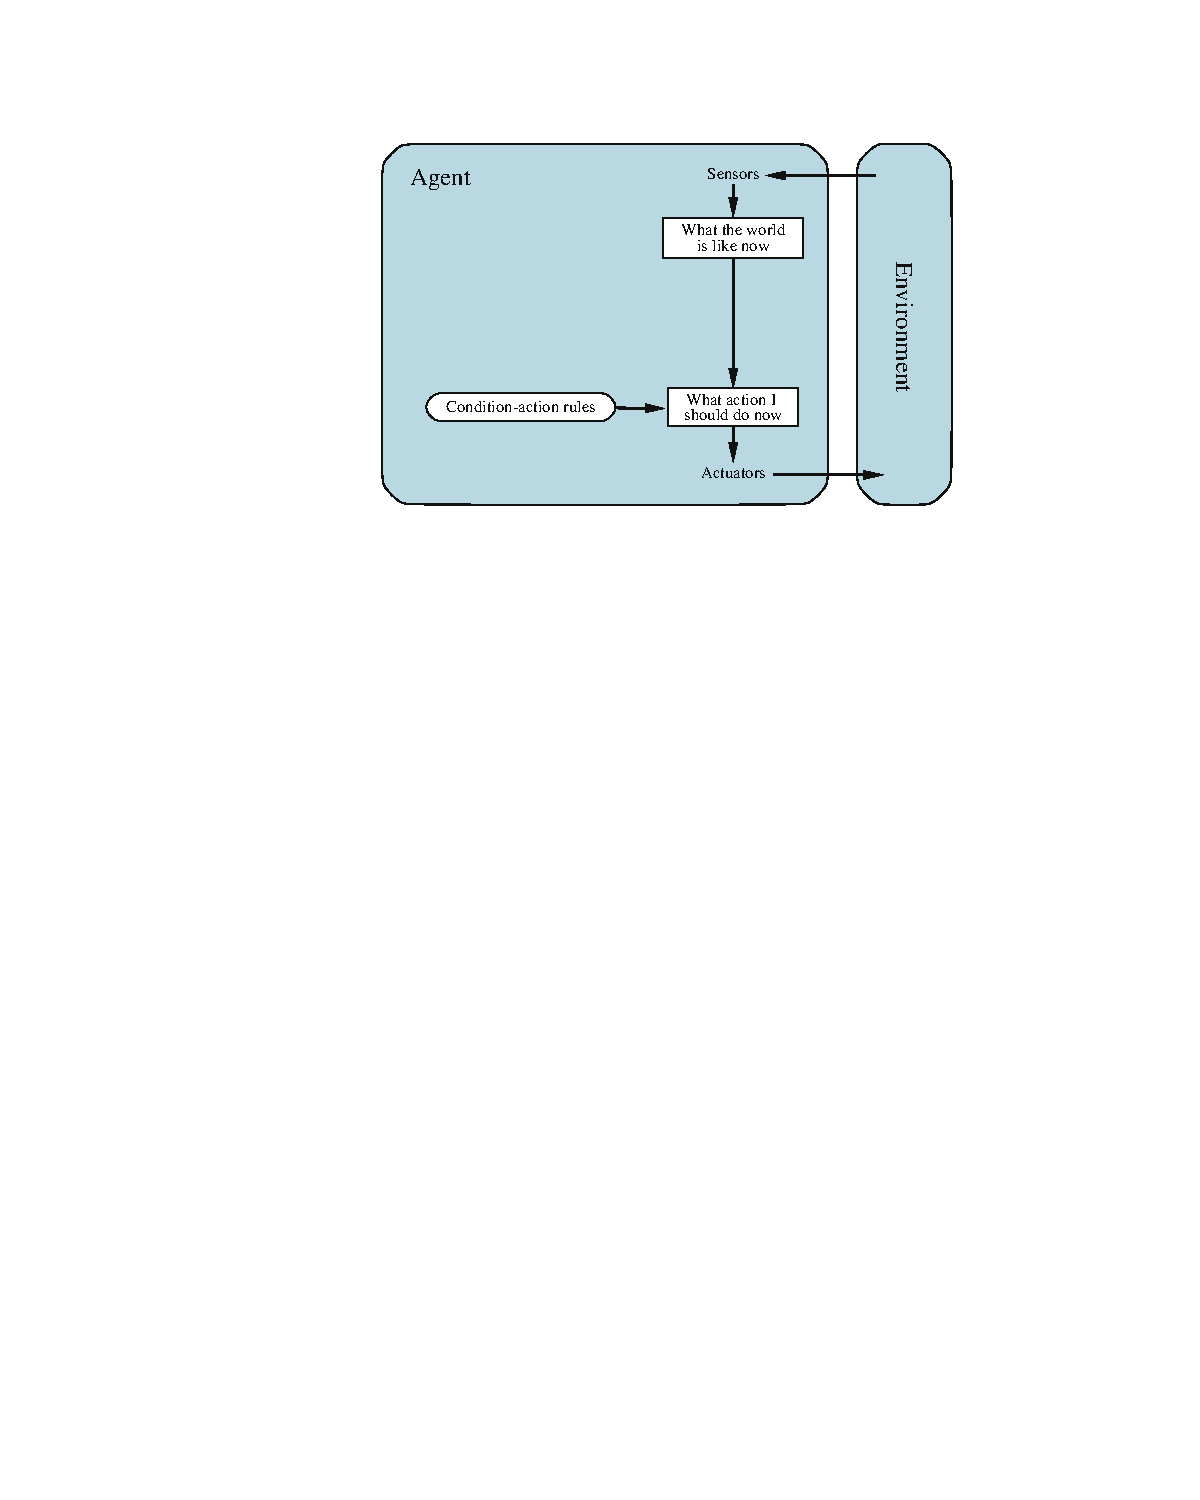
\includegraphics[alt={aima fig 02_09 reflex agent diagram},height=2.0in]{aima-fig-02_09-reflex-agent-diagram.pdf}
\end{flushright}
\section{Condition-Action Rules}
\label{sec:org32e9677}

Condition-action rules (a.k.a. productions or situation-action rules or simply if-then rules) take the form

\begin{itemize}
\item \textbf{if} \textbf{condition} \textbf{then} \textbf{action}
\end{itemize}

\begin{quote}
Simple reflex agents work only if the correct decision can be made on the basis of just the current percept—that is, only if the environment is fully observable.
\end{quote}

Consider the effect of partial observability?

\begin{itemize}
\item What if our reflex vacuum agent has a dirt sensor but no location sensor?
\item How can randomization help?
\end{itemize}
\section{Model-based Agents}
\label{sec:org4eb2a1c}


An agent can keep track of its state by maintaining a \textbf{model} of the environment.  An environment model typically consists of

\begin{itemize}
\item a sensor model, which maps percepts to states, and
\item a state transition model.
\end{itemize}

A transition model typically contains

\begin{itemize}
\item A set of states, \(S\),
\item A set of actions the agent can execute in the environment, \(A\), and
\item A state transition function, \(T(s, a, s')\)
\end{itemize}

Note that the state transition function can be deterministic or nondeterministic.  In most of AI, we consider it to be stochastic.

\begin{equation*}
P(s, a, s') \text{ or } P(s_t \mid s_{t-1}, a_{t-1})
\end{equation*}
\section{Model-based Reflex Agents}
\label{sec:org1a8250d}

\begin{flushleft}
#+latex: 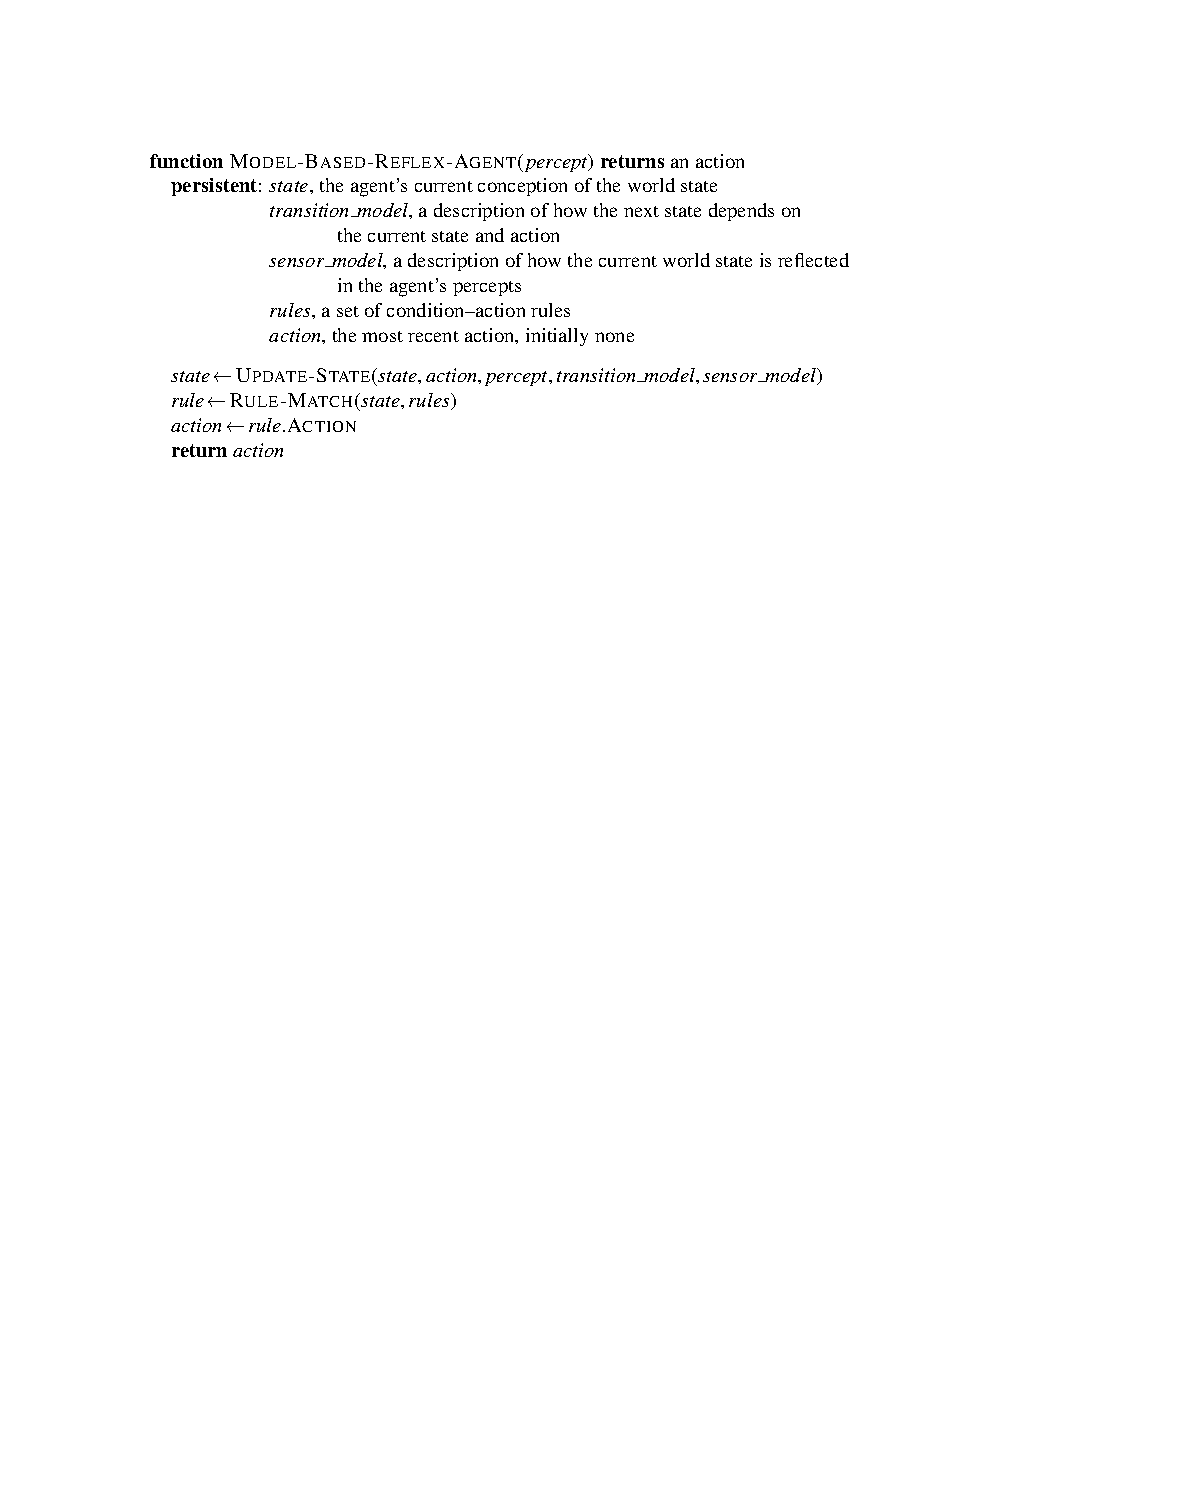
\includegraphics[alt={aima fig 02_12 model based reflex agent program},height=2.0in]{aima-fig-02_12-model-based-reflex-agent-program.pdf}
\end{flushleft}

\vspace{-.3in}
\begin{flushright}
#+latex: 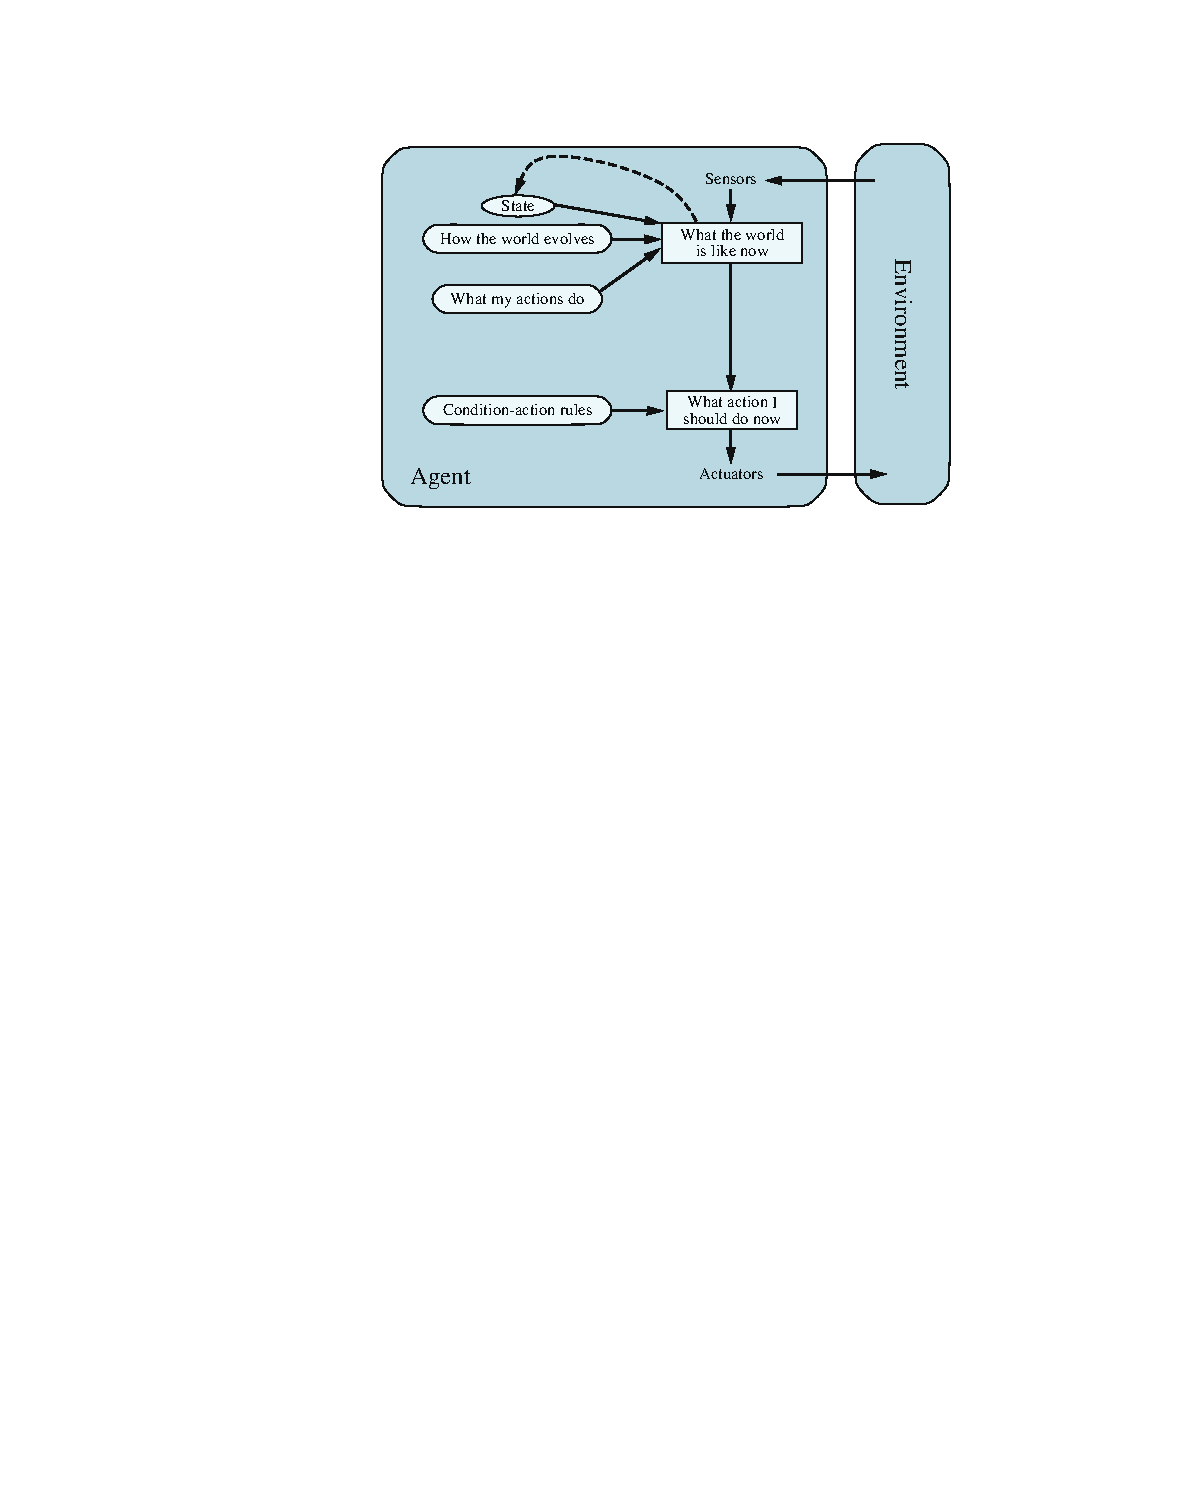
\includegraphics[alt={aima fig 02_11 model based reflex agent diagram},height=1.8in]{aima-fig-02_11-model-based-reflex-agent-diagram.pdf}
\end{flushright}
\section{Model-based Goal-driven Agents}
\label{sec:org4f366d5}


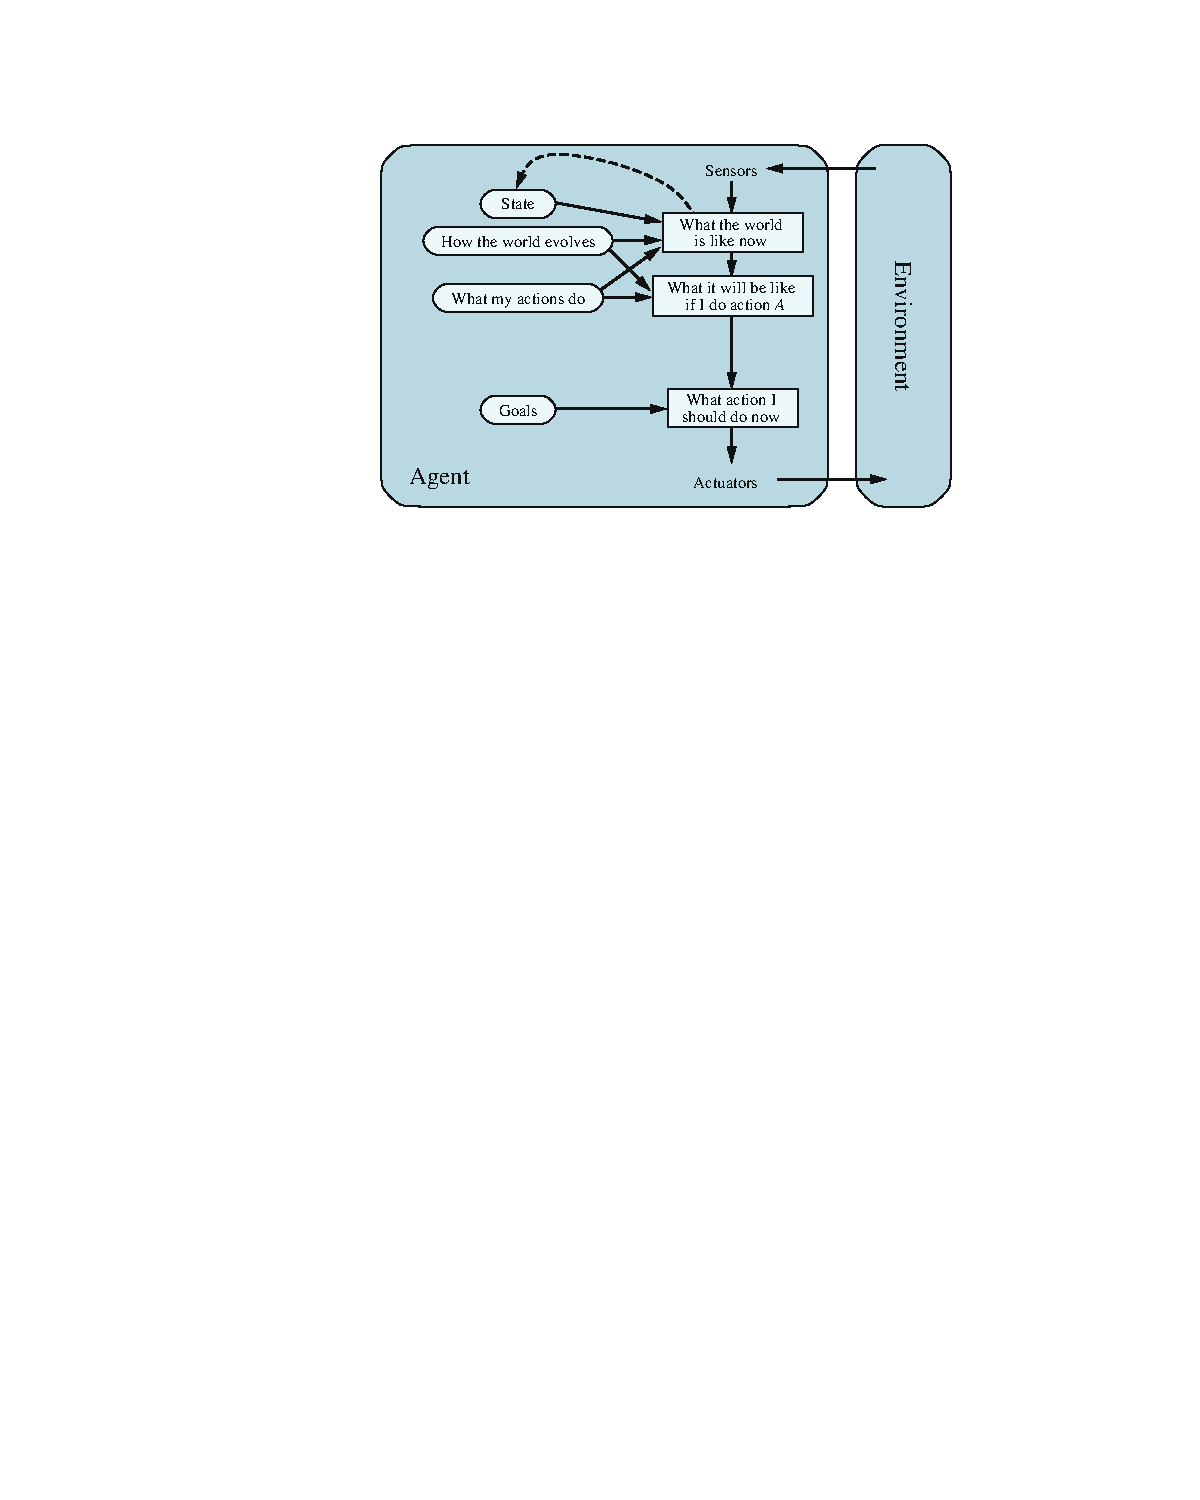
\includegraphics[alt={aima fig 02_13 model based goal driven agent diagram},width=0.75\linewidth]{aima-fig-02_13-model-based-goal-driven-agent-diagram.pdf}


Agents select actions that achieve goals by using \textbf{search} and \textbf{planning} algorithms, which we'll start learning next lecture.
\section{Model-based Utility-driven Agents}
\label{sec:orgc3b2074}


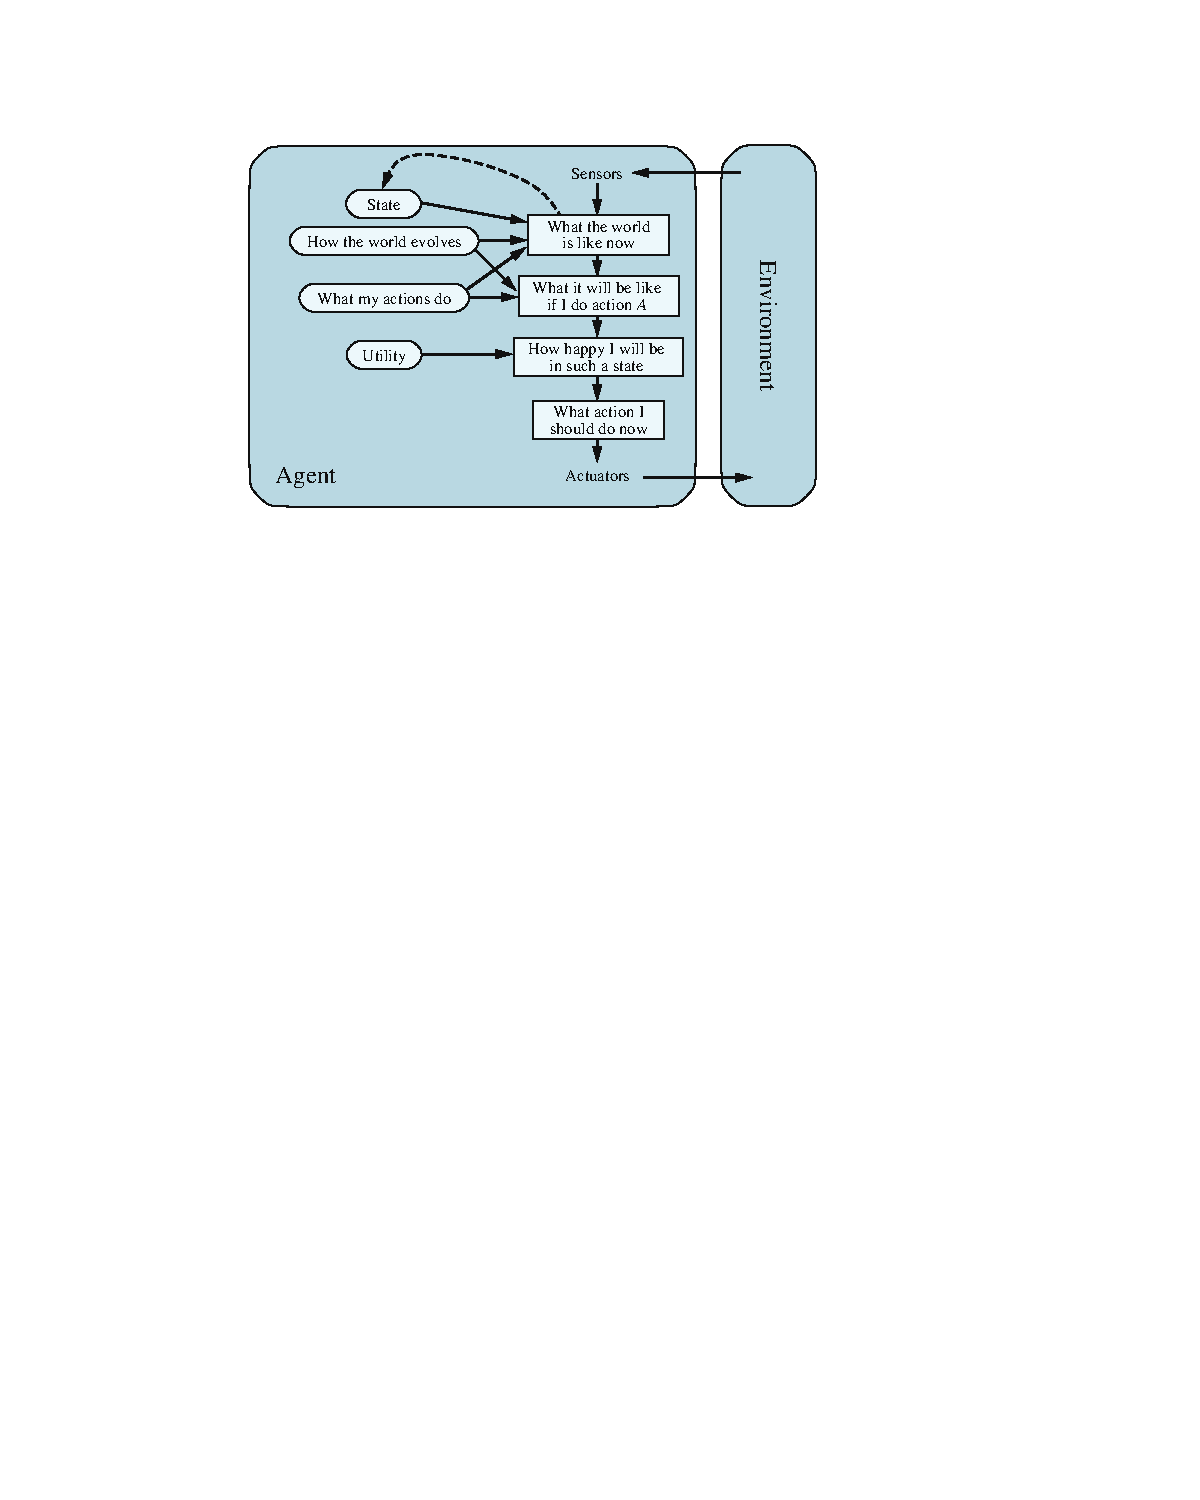
\includegraphics[alt={aima fig 02_14 model based utility driven agent diagram},width=0.75\linewidth]{aima-fig-02_14-model-based-utility-driven-agent-diagram.pdf}


A utility-driven agent seeks states that are more desirable, which is a "soft" way of describing goals.
\section{Learning Agents}
\label{sec:org6b5c7eb}


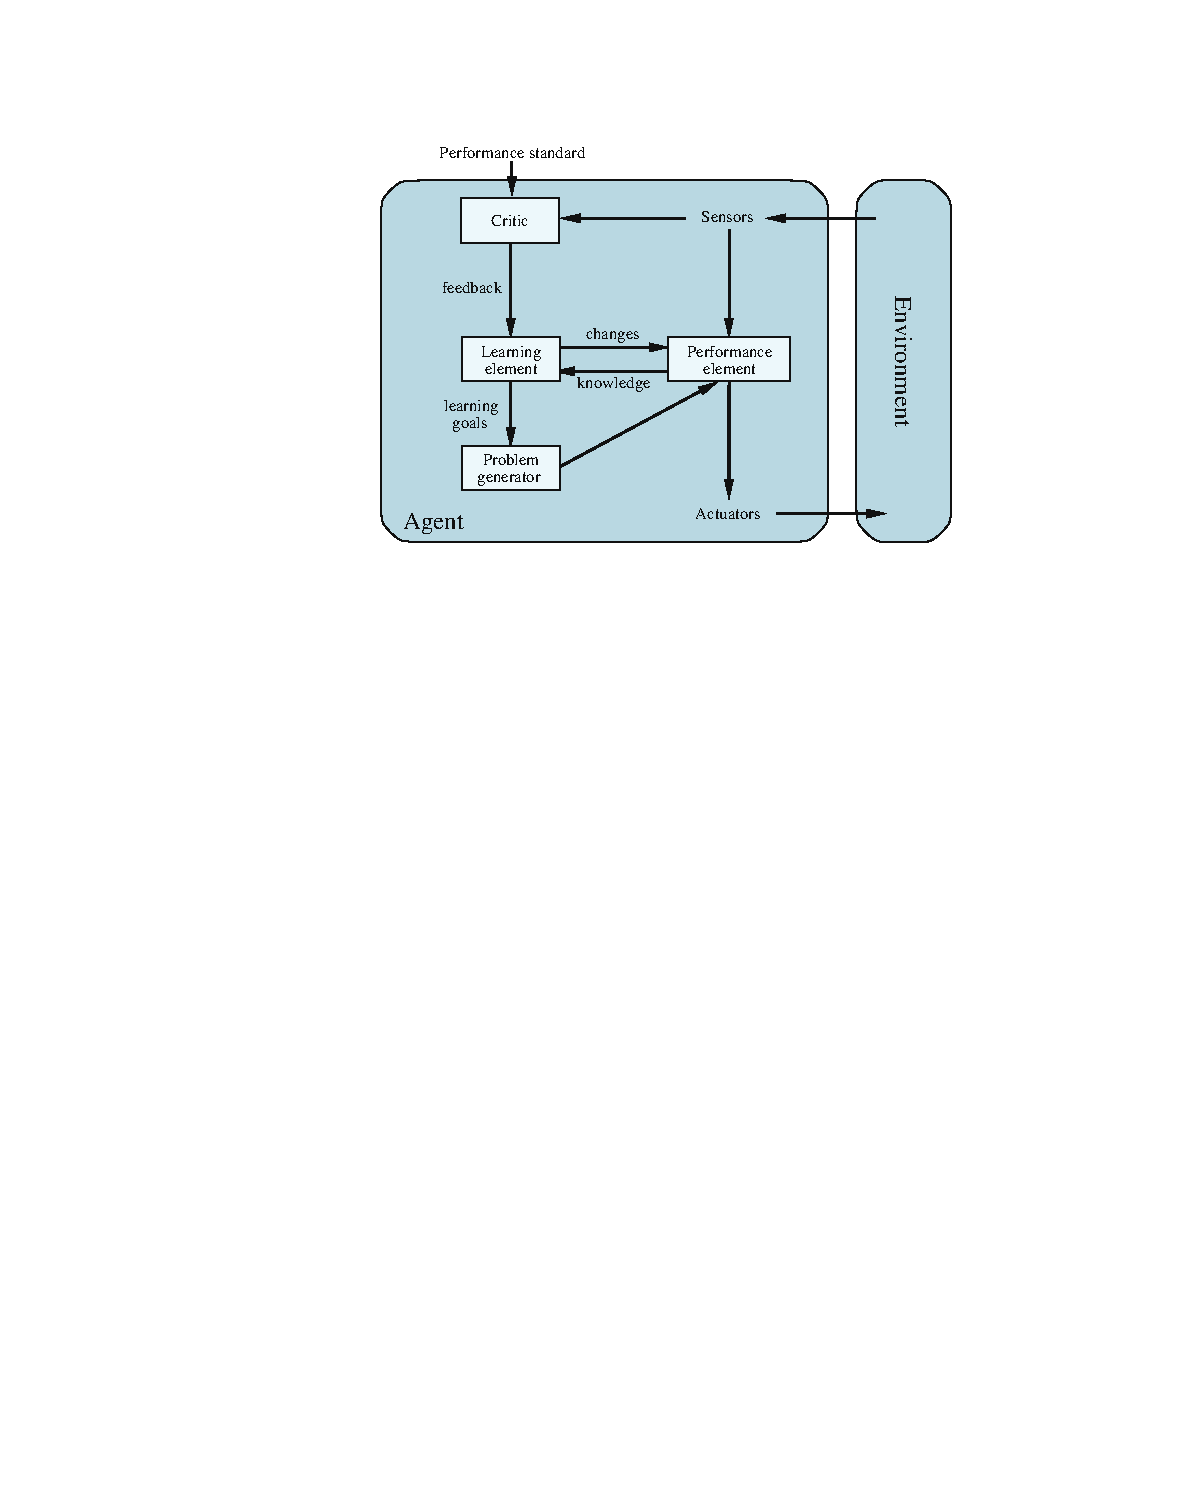
\includegraphics[alt={aima fig 02_15 learning agent diagram},width=0.75\linewidth]{aima-fig-02_15-learning-agent-diagram.pdf}
\section{State Representations}
\label{sec:orga953f86}


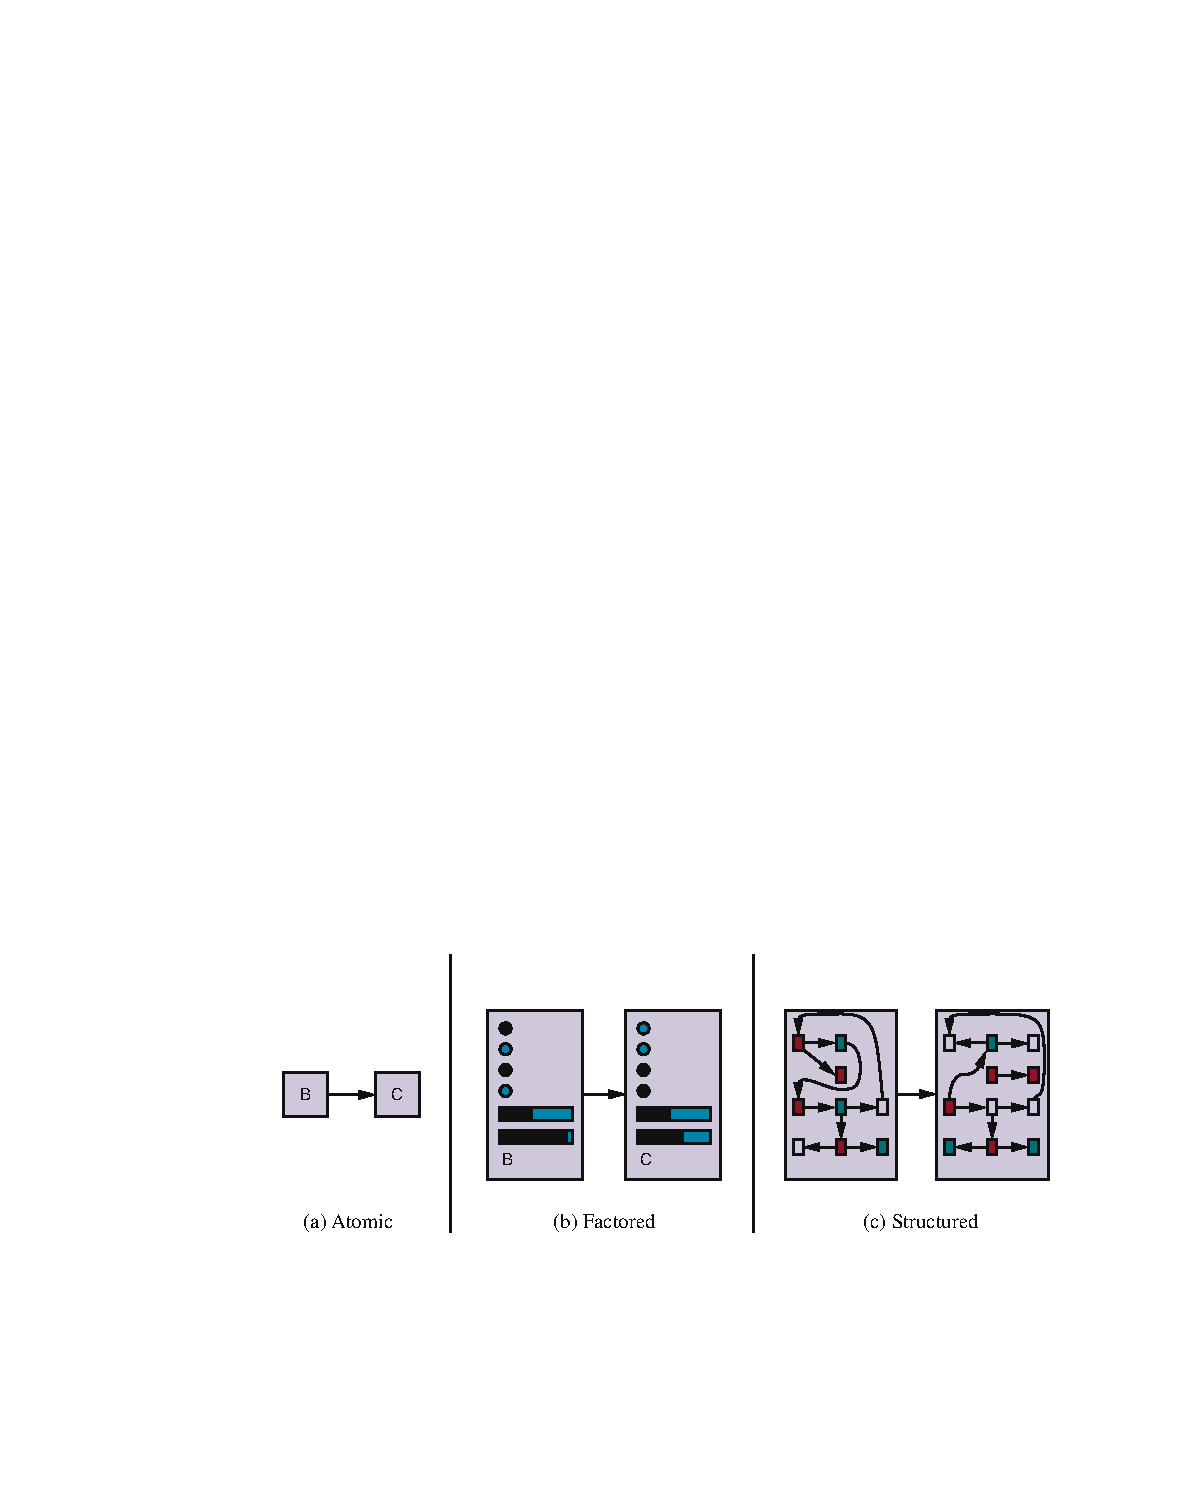
\includegraphics[alt={aima fig 02_16 state representations},width=0.75\linewidth]{aima-fig-02_16-state-representations.pdf}


\begin{itemize}
\item Atomic representations are typically used in search-based problem solving.
\item Factored representations are used in constraint satisfaction, propositional logic, planning, most probabilistic models (e.g., Bayesian networks), and many machine learning algorithms.
\item Structured representations are used in relational databases, first order logic, first-order probability models, and natural language processing.
\end{itemize}
\section{Closing Thoughts}
\label{sec:orgf041cc4}

This lesson has effectively introduced the entire course, providing a framework for everything else we will learn.

\begin{itemize}
\item In the next few lessons we'll learn how to search for right action based on goals.
\item Then we'll learn how to construct knowledge-based models and use them to plan sequences of actions that achieve goals.
\item In the second half of the course we'll learn how to reason under uncertainty, which will help us deal with partial observability.
\item We'll learn how to find optimal actions in multi-agent settings.
\item And we'll learn how to construct the learning elements of agents that improve all of the above with experience.
\end{itemize}
\end{document}
